
\chapter{Results}

\label{chapter:results}

\section{Safety}

\begin{figure}[h!]
    \centering
    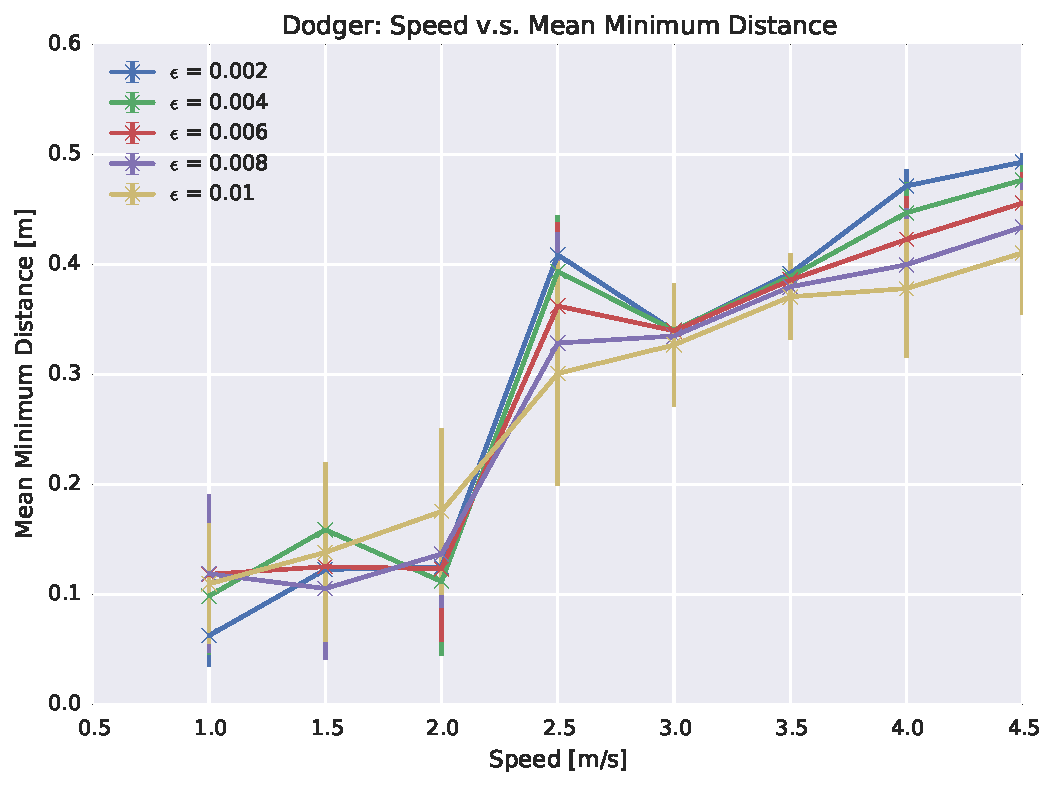
\includegraphics[width=0.48\linewidth]{figs/planner_mean_min_distance_0}
    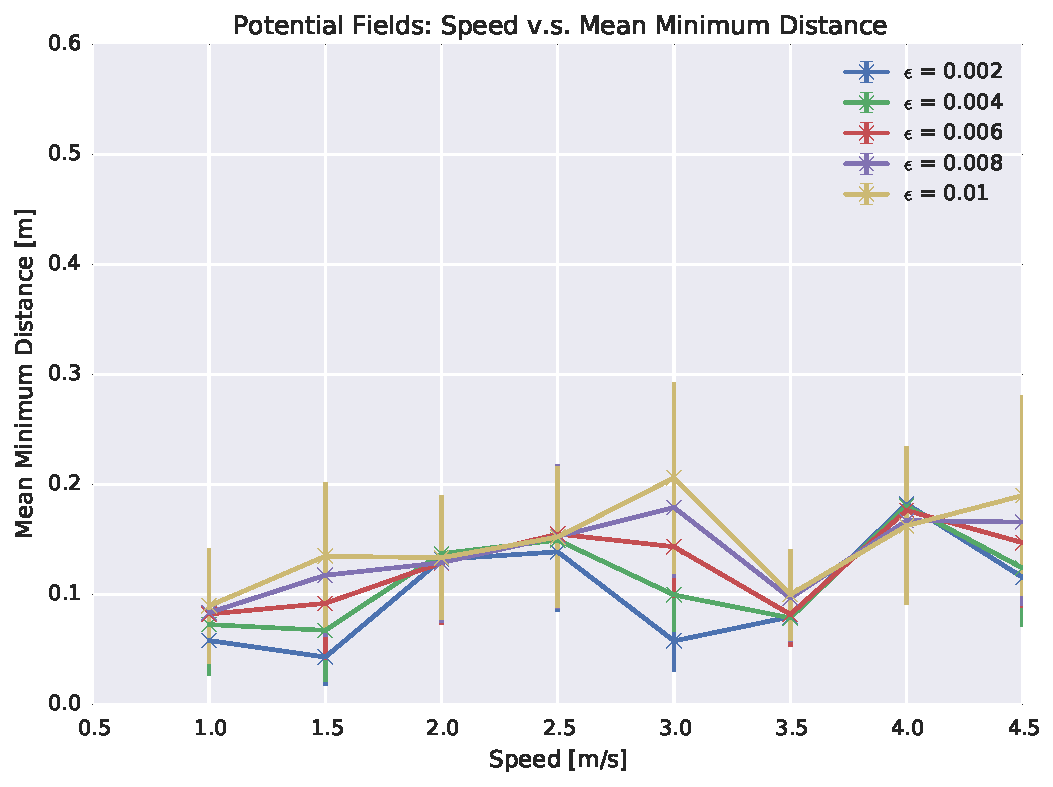
\includegraphics[width=0.48\linewidth]{figs/pf_mean_min_distance_0}
    \caption{Plots showing how the average minimum distance to the obstacles
    changes as the speed increases for various amounts of obstacle position
    uncertainties}
    \label{fig:plot_min_distance}
\end{figure}

\subsection{Variance}

\begin{figure}[h!]
    \centering
    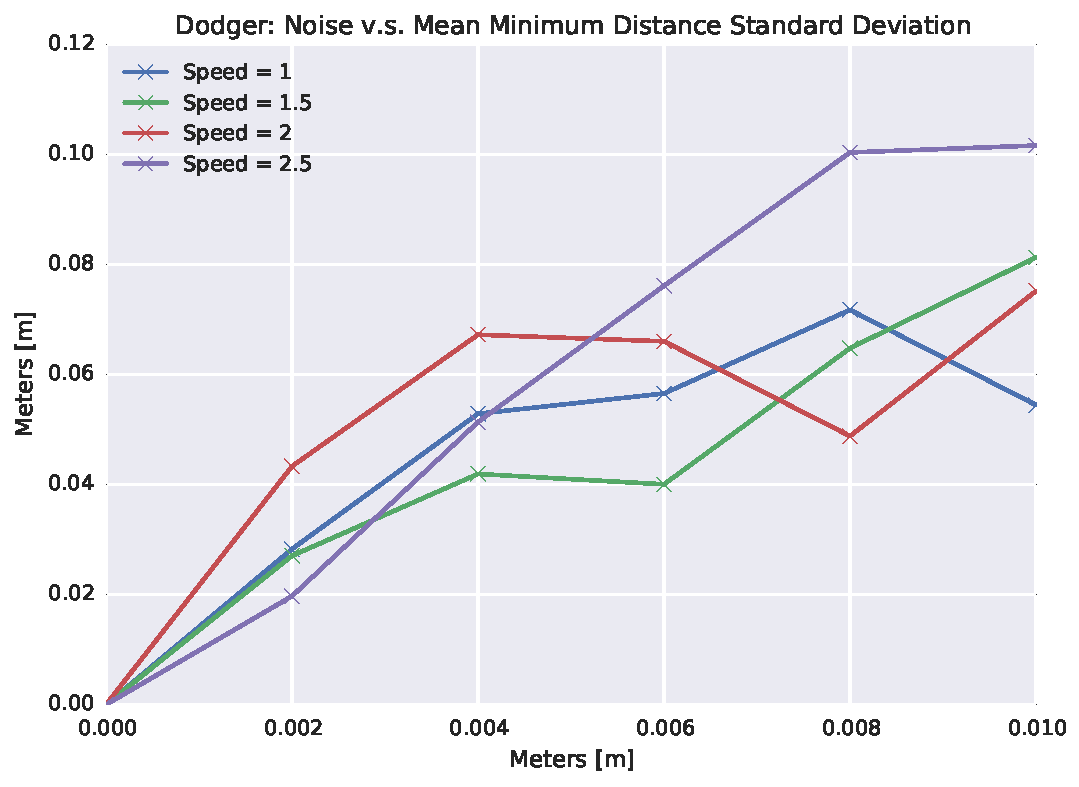
\includegraphics[width=0.48\linewidth]{figs/planner_std_min_distance_0}
    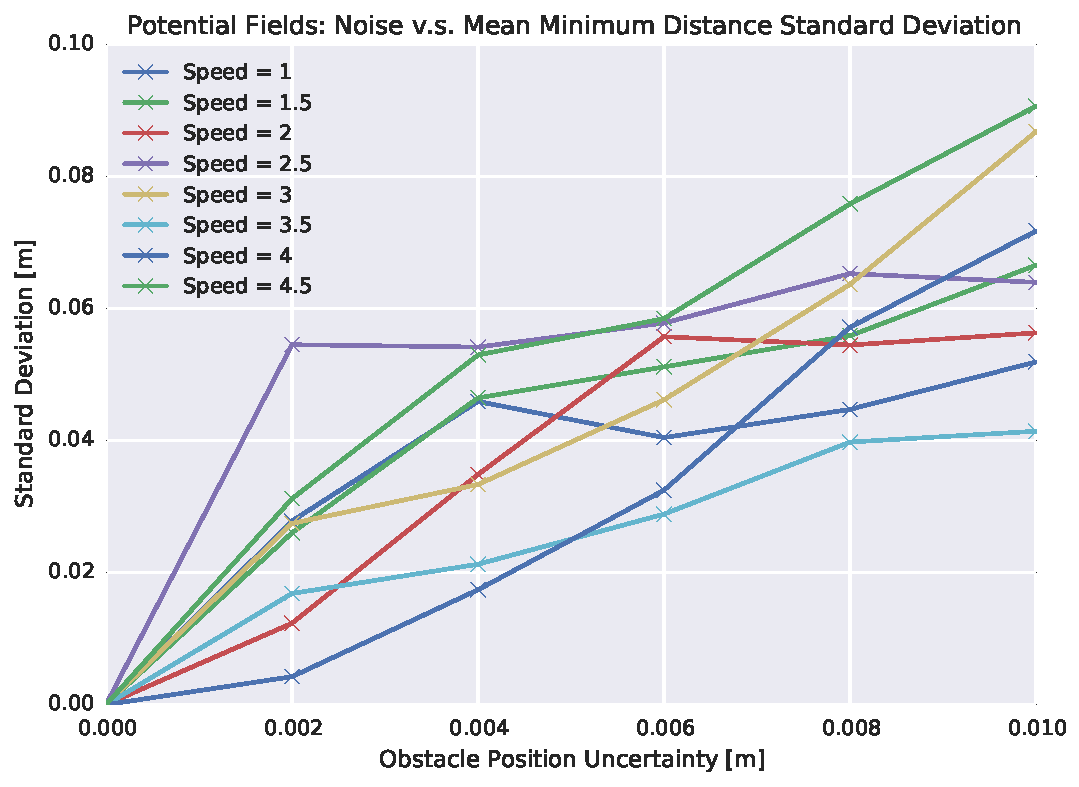
\includegraphics[width=0.48\linewidth]{figs/pf_std_min_distance_0}
    \caption{}
    \label{fig:plot_std_min_distance}
\end{figure}

\section{Computational Time}

\begin{figure}[h!]
    \centering
    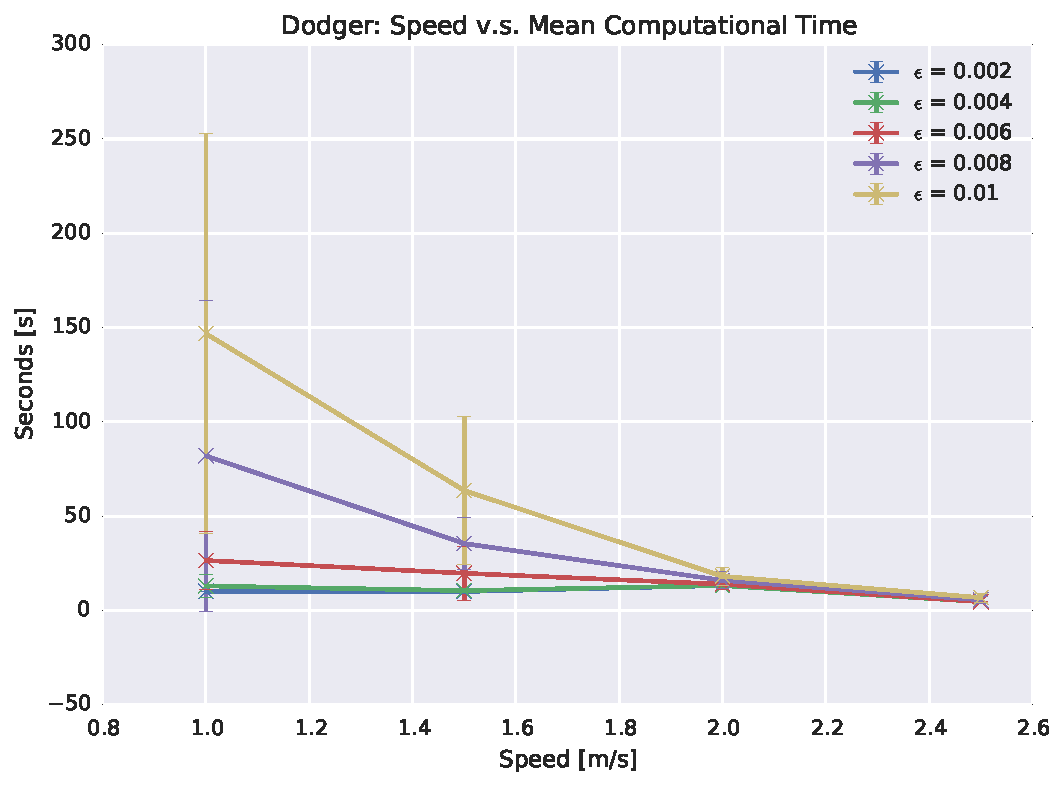
\includegraphics[width=0.48\linewidth]{figs/planner_mean_times_0}
    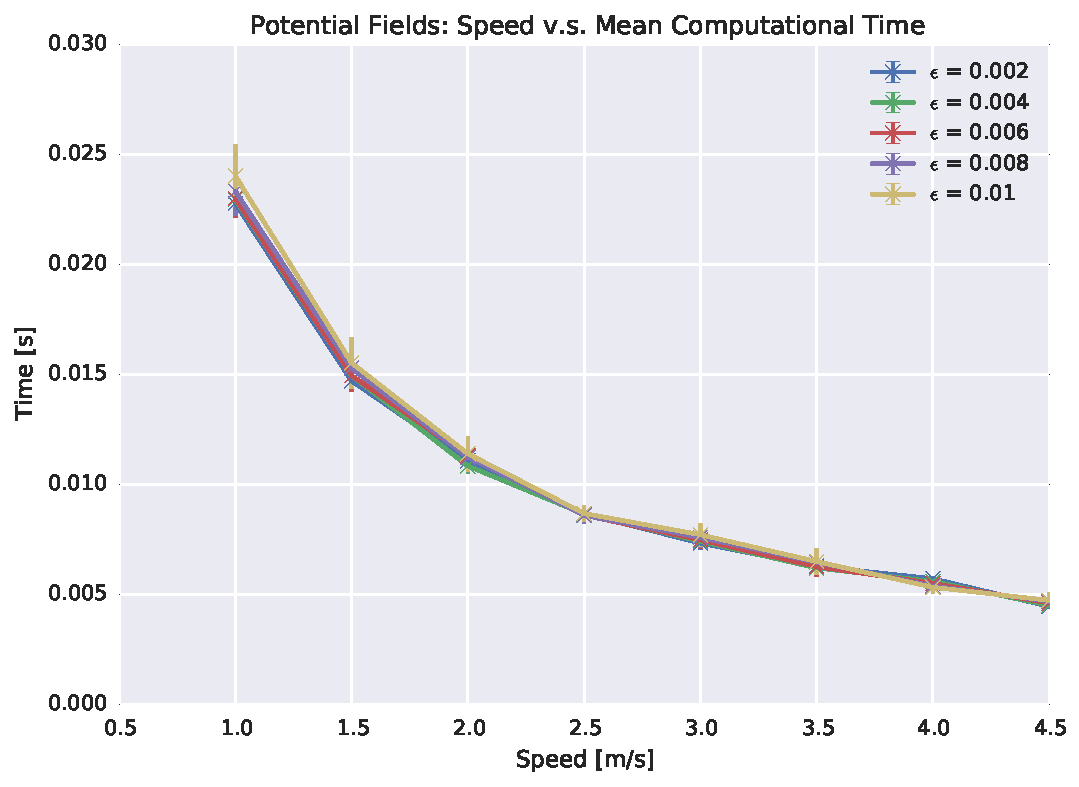
\includegraphics[width=0.48\linewidth]{figs/pf_mean_times_0}
    \caption{Plots showing how the computational time changes as the speed
    increases for various amounts of obstacle position uncertainties}
    \label{fig:plot_comp_time}
\end{figure}

\subsection{Variance}

\begin{figure}[h!]
    \centering
    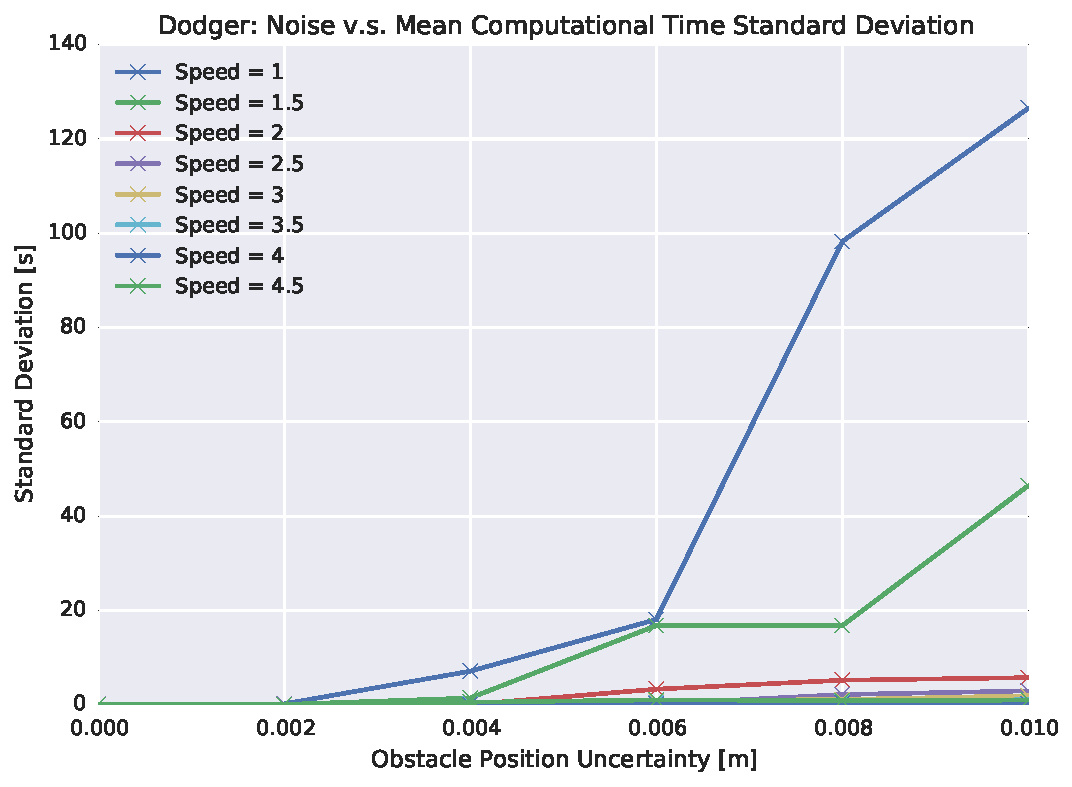
\includegraphics[width=0.48\linewidth]{figs/planner_std_avg_times_0}
    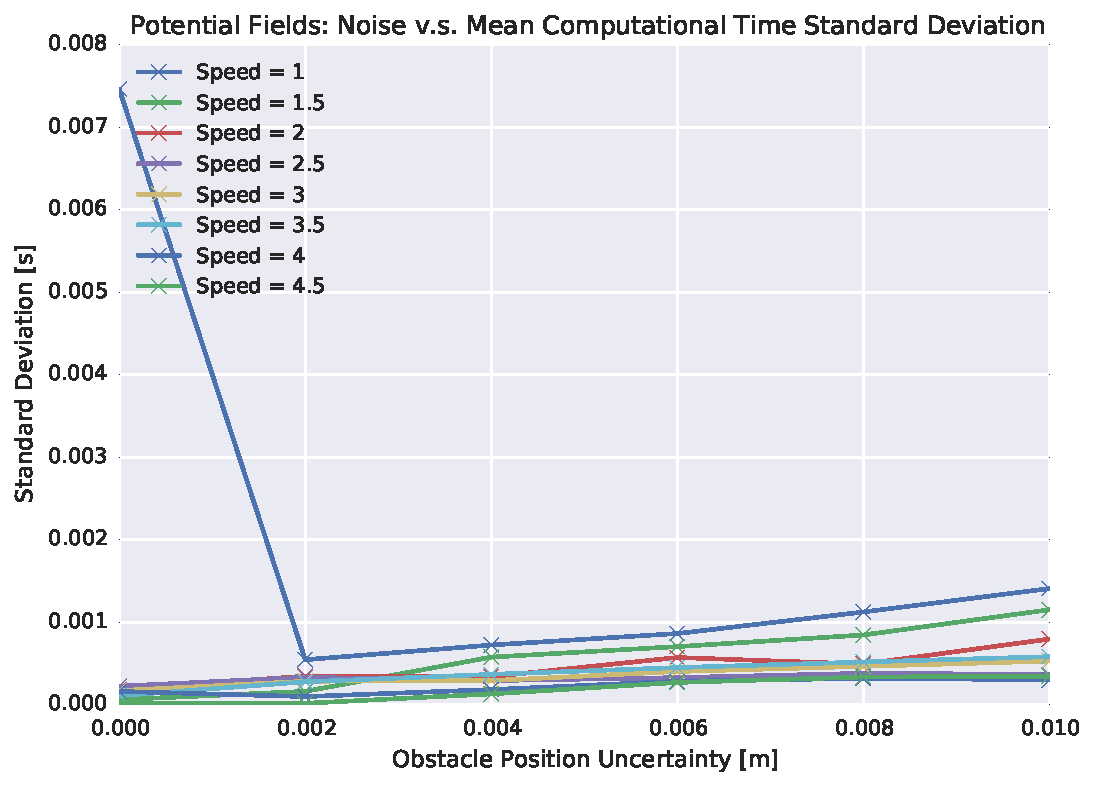
\includegraphics[width=0.48\linewidth]{figs/pf_std_avg_times_0}
    \caption{}
    \label{fig:plot_std_comp_time}
\end{figure}
